\documentclass[letterpaper]{article}
\usepackage[margin=1in]{geometry}
\usepackage[utf8]{inputenc}
\usepackage{textcomp}
\usepackage{amssymb}
\usepackage{natbib}
\usepackage{graphicx}
\usepackage{gensymb}
\usepackage{amsthm, amsmath, mathtools}
\usepackage[dvipsnames]{xcolor}
\usepackage{enumerate}
\usepackage{mdframed}
\usepackage[most]{tcolorbox}
\usepackage{csquotes}
% https://tex.stackexchange.com/questions/13506/how-to-continue-the-framed-text-box-on-multiple-pages

\tcbuselibrary{theorems}

\newcommand{\R}{\mathbb{R}}
\newcommand{\Z}{\mathbb{Z}}
\newcommand{\N}{\mathbb{N}}
\newcommand{\Q}{\mathbb{Q}}
\newcommand{\C}{\mathbb{C}}
\newcommand{\code}[1]{\texttt{#1}}
\newcommand{\mdiamond}{$\diamondsuit$}
\newcommand{\PowerSet}{\mathcal{P}}
\newcommand{\Mod}[1]{\ (\mathrm{mod}\ #1)}
\DeclareMathOperator{\lcm}{lcm}

%\newtheorem*{theorem}{Theorem}
%\newtheorem*{definition}{Definition}
%\newtheorem*{corollary}{Corollary}
%\newtheorem*{lemma}{Lemma}
\newtheorem*{proposition}{Proposition}


\newtcbtheorem[number within=section]{theorem}{Theorem}
{colback=green!5,colframe=green!35!black,fonttitle=\bfseries}{th}

\newtcbtheorem[number within=section]{definition}{Definition}
{colback=blue!5,colframe=blue!35!black,fonttitle=\bfseries}{def}

\newtcbtheorem[number within=section]{corollary}{Corollary}
{colback=yellow!5,colframe=yellow!35!black,fonttitle=\bfseries}{cor}

\newtcbtheorem[number within=section]{lemma}{Lemma}
{colback=red!5,colframe=red!35!black,fonttitle=\bfseries}{lem}

\newtcbtheorem[number within=section]{example}{Example}
{colback=white!5,colframe=white!35!black,fonttitle=\bfseries}{def}

\newtcbtheorem[number within=section]{note}{Important Note}{
        enhanced,
        sharp corners,
        attach boxed title to top left={
            xshift=-1mm,
            yshift=-5mm,
            yshifttext=-1mm
        },
        top=1.5em,
        colback=white,
        colframe=black,
        fonttitle=\bfseries,
        boxed title style={
            sharp corners,
            size=small,
            colback=red!75!black,
            colframe=red!75!black,
        } 
    }{impnote}
\usepackage[utf8]{inputenc}
\usepackage[english]{babel}
\usepackage{fancyhdr}
\usepackage[hidelinks]{hyperref}

\pagestyle{fancy}
\fancyhf{}
\rhead{CSE 101}
\chead{Monday, March 7, 2022}
\lhead{Lecture 23}
\rfoot{\thepage}

\setlength{\parindent}{0pt}

\begin{document}

\section{NP-Completeness}
We continue our discussion on NP-Completeness. 

\subsection{Problem: Circuit SAT}
\textbf{Problem Statement:} Given a circuit $C$ with several Boolean inputs and one Boolean output, determine if there is a set of inputs that give the output \code{1}. 

\bigskip 

For example, the following circuit can be satisfied with inputs $x = y = z = 0$.
\begin{center}
    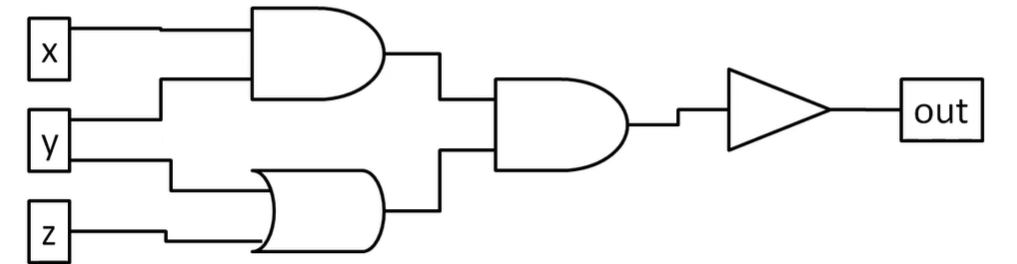
\includegraphics[scale=0.5]{../assets/circuit_sat.png}
\end{center}

\subsubsection{Important Reduction}
Any NP-decision problem can be reduced to Circuit SAT. This is because any NP-decision problem is always of the same form; something is a NP-decision problem if it asks if there is some $X$ that satisfies a polynomial-time checkable property. 

\bigskip 

Essentially, for some polynomial-time computable function $F$, is there an $X$ such that $F(X) = 1$? We can create a circuit $C$ that computes $F$. Then, the problem is equivalent to asking if there is an input for which $C$ outputs 1. So, any NP-decision problem can be encoded as a Circuit SAT problem by taking the function that checks whether or not something satisfies your condition and encoding that as a Boolean circuit. 

\subsubsection{NP-Complete}
Circuit-SAT is our first example of an \textbf{NP-Complete} problem. This is a problem in NP that is at \emph{least} as hard as any other problem in NP. Therefore: 
\begin{itemize}
    \item If we can find a polynomial time algorithm that can solve Circuit SAT, we have a polynomial time algorithm for \emph{all} NP problems. 
    \item However, if any problem in NP is hard, then Circuit SAT is \emph{hard}.
\end{itemize}
\textbf{Remark:} Decision problems can be NP-Complete. For optimization problems, we call them NP-Hard.

\subsubsection{Other NP-Complete/Hard Problems}
We note that the following problems are all NP-Complete or NP-Hard: 
\begin{itemize}
    \item Formula SAT. 
    \item Maximum Independent Set. 
    \item Traveling Salesman Problem. 
    \item Hamiltonian Cycle. 
    \item Generalized Knapsack. 
\end{itemize}
We can show this by finding reductions from other NP-Hard or NP-Complete problems. 

\subsubsection{3-SAT}
3-SAT is a special case of formula-SAT where the formula is an \code{AND} of clauses and each clause is an \code{OR} of at most 3 variables or their negations. The following is an example of a 3-SAT problem: 
\[(x \lor y \lor z) \land (\overline{x} \lor u) \land (w \lor \overline{z} \lor u) \land (\overline{u} \lor w \lor \overline{z}) \land (\overline{y})\]
Here, each clause has \emph{at most three} variables or their negations. Each clause only has \code{OR} operations, and each clause is separated by \code{AND} operations. 

\subsubsection{Showing that 3-SAT is NP-Complete}
We will show that 3-SAT is NP-Complete. This is done by reducing Circuit-SAT to 3-SAT. 
\begin{itemize}
    \item Let's suppose we start with a circuit from a circuit-SAT problem. 
    \begin{center}
        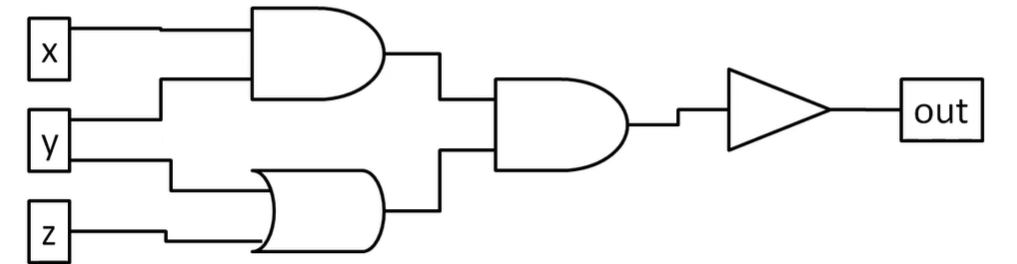
\includegraphics[scale=0.4]{../assets/circuit_sat.png}
    \end{center}

    \item Next, we'll create new variables for each outgoing wire.
    \begin{center}
        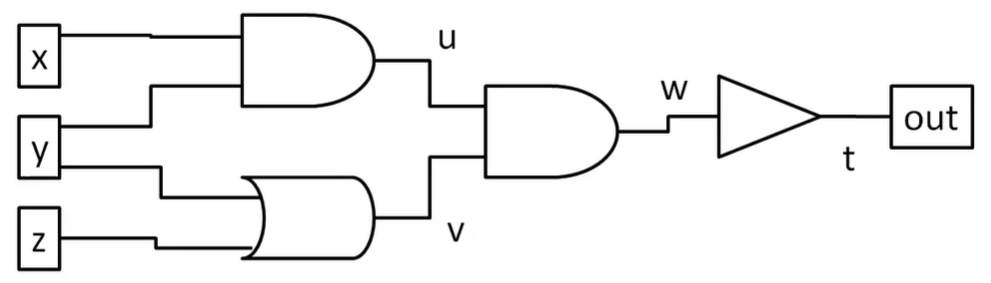
\includegraphics[scale=0.4]{../assets/circuit_sat_2.png}
    \end{center}

    \item For each variable, we'll create a formula for each gate and for the output. We know that output $t$ must be true. Then, each clause is defined by its variables and the output after performing some operation (e.g. $x$ and $y$ are the inputs to the \code{AND} gate and $u$ is the output). Thus, we can write the formula out like so: 
    \[(v \iff y \lor z) \land (u \iff x \land y) \land (w \iff u \land v) \land (t \iff \overline{w}) \land t\]

    \item Note that the formula above is \emph{not} a 3-SAT formula. Effectively, we have 3-variable clauses that aren't 3-SAT clauses, so the goal is to write it in terms of them. 
    \begin{mdframed}[]
        To write thes 3-variable clauses in a way that represents 3-SAT clauses, we write out a truth table for each clause. Note that this is just an example of how you would do this.
        
        \bigskip 

        For example, consider a clause $(z \iff x \lor y)$. There are 8 different possibilities for all combinations of $x$, $y$, and $z$. For each combination of the original statement, we fill out the table like so. 
        \begin{center}
            \begin{tabular}{|c|c|c|c|}
                \hline 
                $x$ & $y$ & $z$ & $z \iff x \lor y$ \\ 
                \hline 
                0 & 0 & 0 & 1 \\ 
                0 & 0 & 1 & 0 \\ 
                0 & 1 & 0 & 0 \\ 
                0 & 1 & 1 & 1 \\ 
                1 & 0 & 0 & 0 \\ 
                1 & 0 & 1 & 1 \\ 
                1 & 1 & 0 & 0 \\ 
                1 & 1 & 1 & 1 \\ 
                \hline 
            \end{tabular}
        \end{center}
        We note that when we impose a 3-SAT clause on three variables, it excludes exactly \emph{one} combination of the inputs. We now describe how this works specifically. The idea is, given the original truth table of each clause:
        \begin{itemize}
            \item Find all rows where the result is \code{0}. In our initial example, we have 
            \begin{center}
                \begin{tabular}{|c|c|c|c|}
                    \hline 
                    $x$ & $y$ & $z$ & $z \iff x \lor y$ \\ 
                    \hline 
                    0 & 0 & 1 & 0 \\ 
                    0 & 1 & 0 & 0 \\ 
                    1 & 0 & 0 & 0 \\ 
                    1 & 1 & 0 & 0 \\ 
                    \hline 
                \end{tabular}
            \end{center}
    
            \item Then, for each row, negate the correct inputs so that the result would be \code{0} in the parameters; then, \code{OR} each of them. So, for example, with the first row, you would have $x \lor y \lor \overline{z}$. This is because $x$'s original value was \code{0}, so you would use $x$ in the 3-SAT instance to ``keep'' the \code{0}. Likewise, since $z$'s original value is \code{1}, you would use $\overline{z}$ to negate the \code{1} to a \code{0}. 
            \item For each of the remaining rows, do the same thing. Combine the clauses with an \code{AND} operator. For example, with the second row, we would have $x \lor \overline{y} \lor z$. Then, we can combine this with the previous step by using the \code{AND} operator like so: 
            \[(x \lor y \lor \overline{z}) \land (x \lor \overline{y} \lor z)\]
            Eventually, you'll end up with the 3-SAT-equivalent of the above expression:
            \[\underbrace{(x \lor y \lor \overline{z})}_{\text{1st Row}} \land \underbrace{(x \lor \overline{y} \lor z)}_{\text{2nd Row}} \land \underbrace{(\overline{x} \lor y \lor z)}_{\text{3rd Row}} \land \underbrace{(\overline{x} \lor \overline{y} \lor z)}_{\text{4th Row}} = (z \iff x \lor y)\]
            \item Repeat this process for each of the clauses that needs to be converted. 
        \end{itemize}
    \end{mdframed}

    \item This means that 3-SAT is also NP-Complete since any problem in NP can be reduced to Circuit-SAT, which in turn can be reduced to 3-SAT.
\end{itemize}

\subsubsection{Another Look at 3-SAT}
\begin{lemma}{}{}
    A 3-SAT instance is satisfiable if and only if it is possible to select one term from each clause without selecting both a variable and its negation. 
\end{lemma}

For example, suppose we have the 3-SAT instance 
\[(x \lor y \lor z) \land (\overline{x} \lor y) \land (\overline{y} \lor \overline{z}) \land (\overline{x} \lor z)\]
For each clause, suppose we select one of the terms like so.  
\[(x \lor \boxed{y} \lor z) \land (\boxed{\overline{x}} \lor y) \land (\overline{y} \lor \boxed{\overline{z}}) \land (\boxed{\overline{x}} \lor z)\]
We note that we did not select both a variable and its negation (e.g. we didn't select an $x$ and $\overline{x}$). This shows that this 3-SAT instance is satisfiable. For this example, if $x = \text{False}$, $y = \text{True}$, and $z = \text{False}$, then this statement will be \text{True}.

\begin{mdframed}[]
    \begin{proof}
        Suppose the instance was satisfiable. Then, at least one term in each clause must be true since each clause consists of \code{OR} of some number of terms. We select one such term from each clause. We note that they cannot contradict each other since all of those terms are consistent with the same satisfying assignment (it can't be true that $x$ was true in one clause and $\overline{x}$ was true in another clause because $x$ had to either be true or false).

        \bigskip 

        Suppose we have a 3-SAT instance where we can select one term from each clause without selecting both a variable and its negation. Suppose we set those clauses to be true (for example, we can set $x$ to be True and $y$ to be False or whatever so each clause is true). Then, we set the other variables arbitrarily since we know that at least one variable in each clause is true. This causes the whole statement to be true. 
    \end{proof}
\end{mdframed}

\subsubsection{Reducing 3-SAT to Maximum Independent Set}
This reduction is interesting especially since these problems appear to be unrelated. So, we start with a new formulation of 3-SAT. We want to select one term from each clause. We note that: 
\begin{itemize}
    \item For 3-SAT, we have a bunch of terms and we want to select some of them. 
    \item For MIS, we have a bunch of vertices and we want to select some of them. 
\end{itemize}
Suppose we want to reduce the following 3-SAT instance to a Maximum Independent Set instance.
\[(x \lor y \lor z) \land (\overline{x} \lor y) \land (\overline{y} \lor \overline{x})\]
This is how you would go about it. 
\begin{itemize}
    \item First, for each term in each clause, create a vertex.
    \begin{center}
        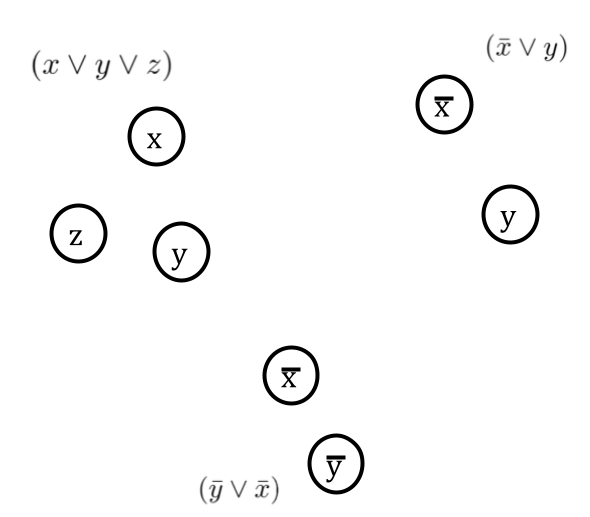
\includegraphics[scale=0.4]{../assets/3sat_mis_1.png}
    \end{center}

    \item We now need to add edges in the following way. 
    \begin{itemize}
        \item First, we want to add edges between terms in the same clause.
        \begin{center}
            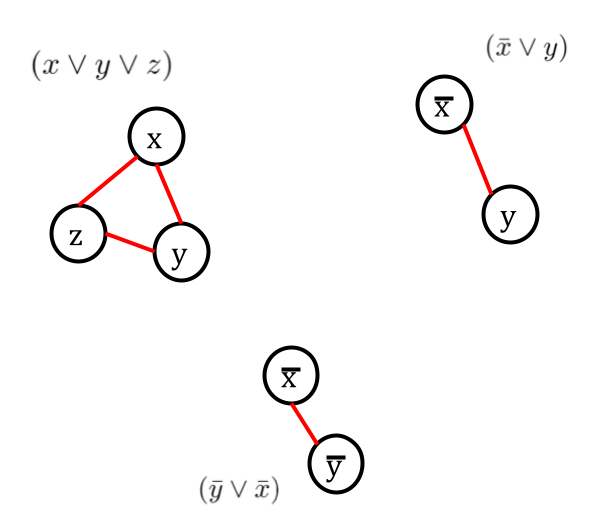
\includegraphics[scale=0.4]{../assets/3sat_mis_2.png}
        \end{center}
        These edges ensure that, if we pick an independent set, we can only pick one term from each clause. 

        \item We add edges between contradictory terms.
        \begin{center}
            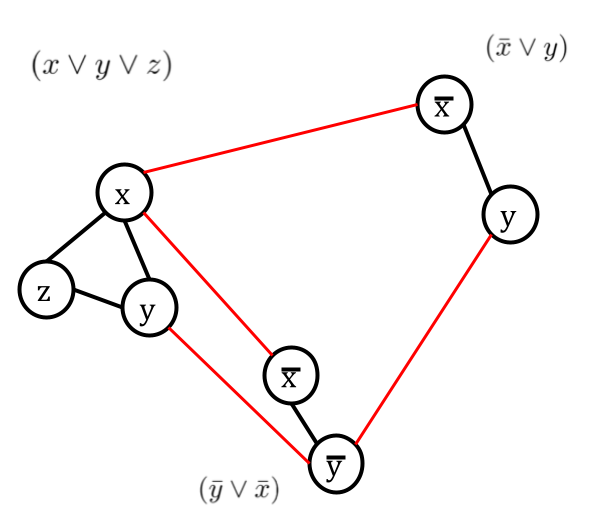
\includegraphics[scale=0.4]{../assets/3sat_mis_3.png}
        \end{center}
        For example, we add an edge between the vertex $x$ and a vertex $\overline{x}$. 
    \end{itemize}
    This gives us the graph that we can use for the Maximum Independent Set instance. 
\end{itemize}

We note that an independent set in this graph has: 
\begin{itemize}
    \item At most one vertex from each clause. 
    \item No pair of vertices corresponding to contradictory terms. 
\end{itemize}
This is because of the edges; an independent set is not allowed to have two vertices connected by an edge. Since two things in the same clause are connected by an edge, it can't have two things in the same clause. And since two contradictory things are connected by an edge, it cannot have two contradictory things. Other than that, it can have whatever vertices it wants. 

\bigskip 

In particular, can we find an independent set such that its size is the same as the number of clauses in the original 3-SAT expression? If we can, then the only way to do that, since we can't select more than one vertex per clause, is if we pick exactly one vertex per clause. Additionally, because of the second contradict, we had to have done this without any pair that contradicts each other. This is exactly what we need to find a satisfying assignment for the 3-SAT. The opposite direction works as well; if we can satisfy the 3-SAT, we can pick one vertex from each clause and that will give us an independent set of the corresponding graph of the appropriate size. 

\bigskip 

So, to summarize the previous paragraph, we note that we have an independent set of size $c$ (where $c$ is the number of clauses) if and only if you can select one term from each clause without a contradicton. Therefore, the size of the maximum independent set is equal to the number of clauses if and only if the 3-SAT has a solution. 

\subsubsection{Example of Reducing 3-SAT to MIS}
Consider the graph we created in the previous section. If we select the following vertices (the pink vertices): 
\begin{center}
    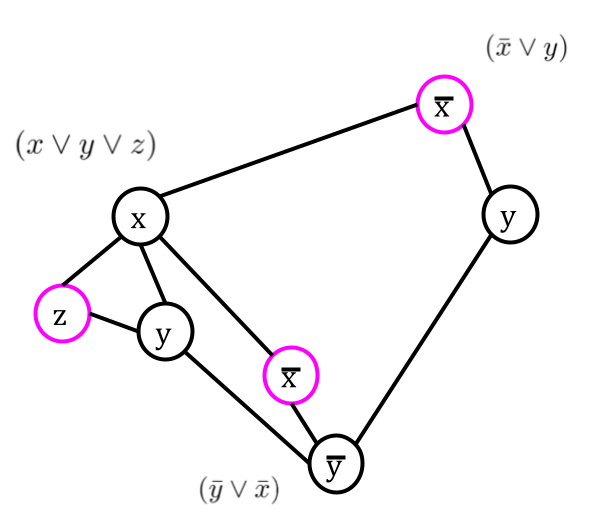
\includegraphics[scale=0.4]{../assets/3sat_mis_4.png}
\end{center}
Then, as long as $x = \text{False}$, $z = \text{True}$, and $y$ is arbitrary, then we found a satisfying assignment. 


\subsection{Problem: Zero-One Equations}
To prove more complicated reductions, it is helpful to have the correct problem to prove the reductions from. Sometimes, you might need to build intermediate problems that are nice to work with, mainly for convenience. 

\bigskip 

One convenient problem is the \textbf{zero-one equation}. Given a matrix $A$ with only \code{0}'s and \code{1}'s as entries and a vector $b$ of only \code{1}'s, determine whether or not there is an $x$ with \code{0} and \code{1} entries so that 
\[Ax = b\]
The problem is clearly in NP. We will show that is NP-complete. 

\subsubsection{Example: Zero-One Equations}
Find an $x_1, x_2, x_3$ such that 
\[\begin{bmatrix}
    1 & 0 & 1 \\ 1 & 1 & 0
\end{bmatrix} \begin{bmatrix}
    x_1 \\ x_2 \\ x_3
\end{bmatrix} = \begin{bmatrix}
    1 \\ 1
\end{bmatrix}\]
is satisfied. Equivalently, does there exist $x_1, x_2, x_3 \in \{0, 1\}$ such that 
\[\begin{cases}
    x_1 + x_3 = 1 \\ 
    x_1 + x_2 = 1
\end{cases}\]
holds? 

\begin{mdframed}[]
    It's not hard to see that this holds.     
\end{mdframed}

Generally, this is what a zero-one equation looks like; a bunch of sets of $x_i$'s that need to add to \code{1}. 


\end{document}